In this experiment we considered two different curves \(q\) and \(r\) with SRVT forms
\begin{equation*}
    q(t) = [\cos(t), \sin(t)], \quad  r(t) = [0,1]. 
\end{equation*}
The corresponding optimal reparametrization problem has an analytical solution computed in \cite[A.1]{woien2019} and given by 
\begin{equation*}
    \varphi(t) = t - \frac{\sin(2 \pi t)}{2 \pi}.
\end{equation*}

\begin{figure}[b]
    \begin{subfigure}[t]{0.5\textwidth}
        \centering
        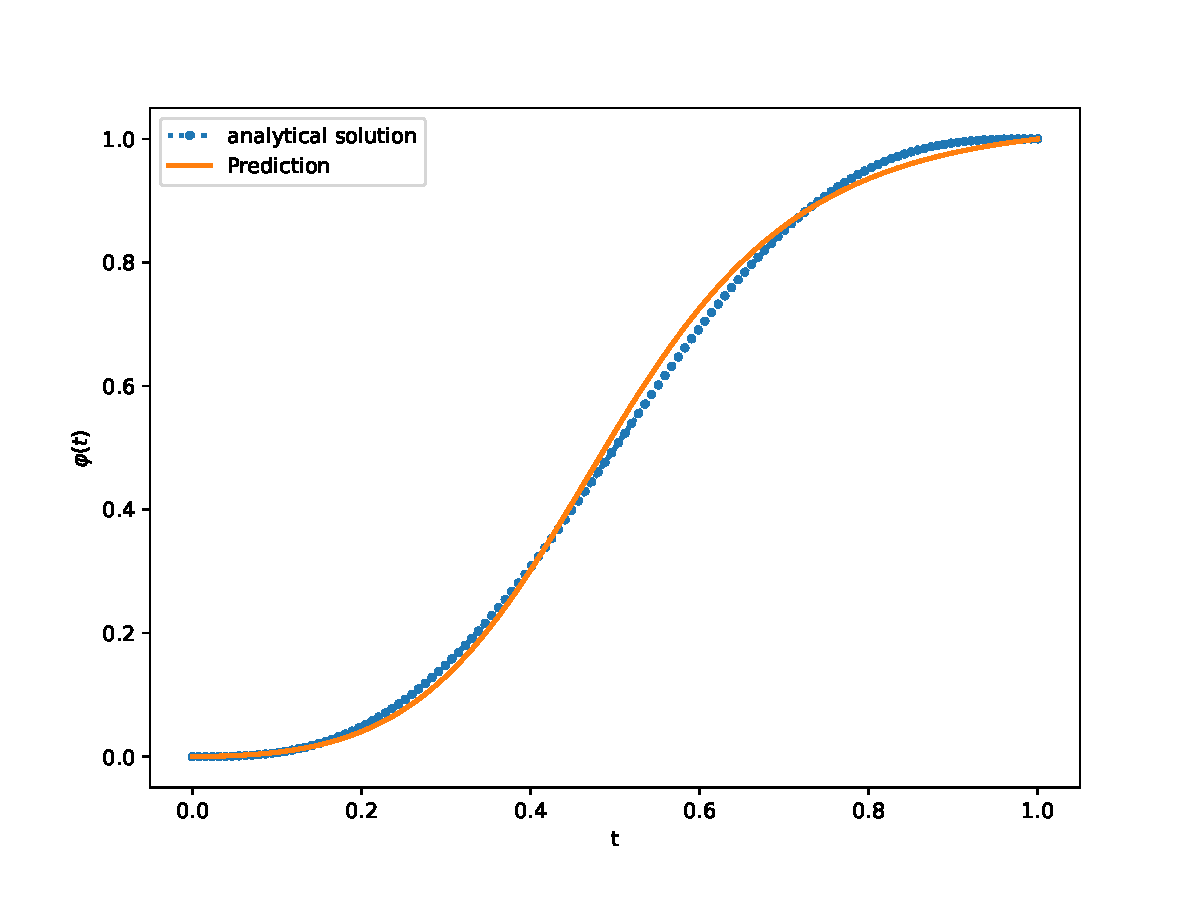
\includegraphics[width=\linewidth]{figures/curve_2/exp_3/plot_0_0.pdf}
        \caption{The approximate optimal reparametrization}\label{fig:curve_2_solution}
    \end{subfigure}
    \begin{subfigure}[t]{0.5\textwidth}
        \centering
        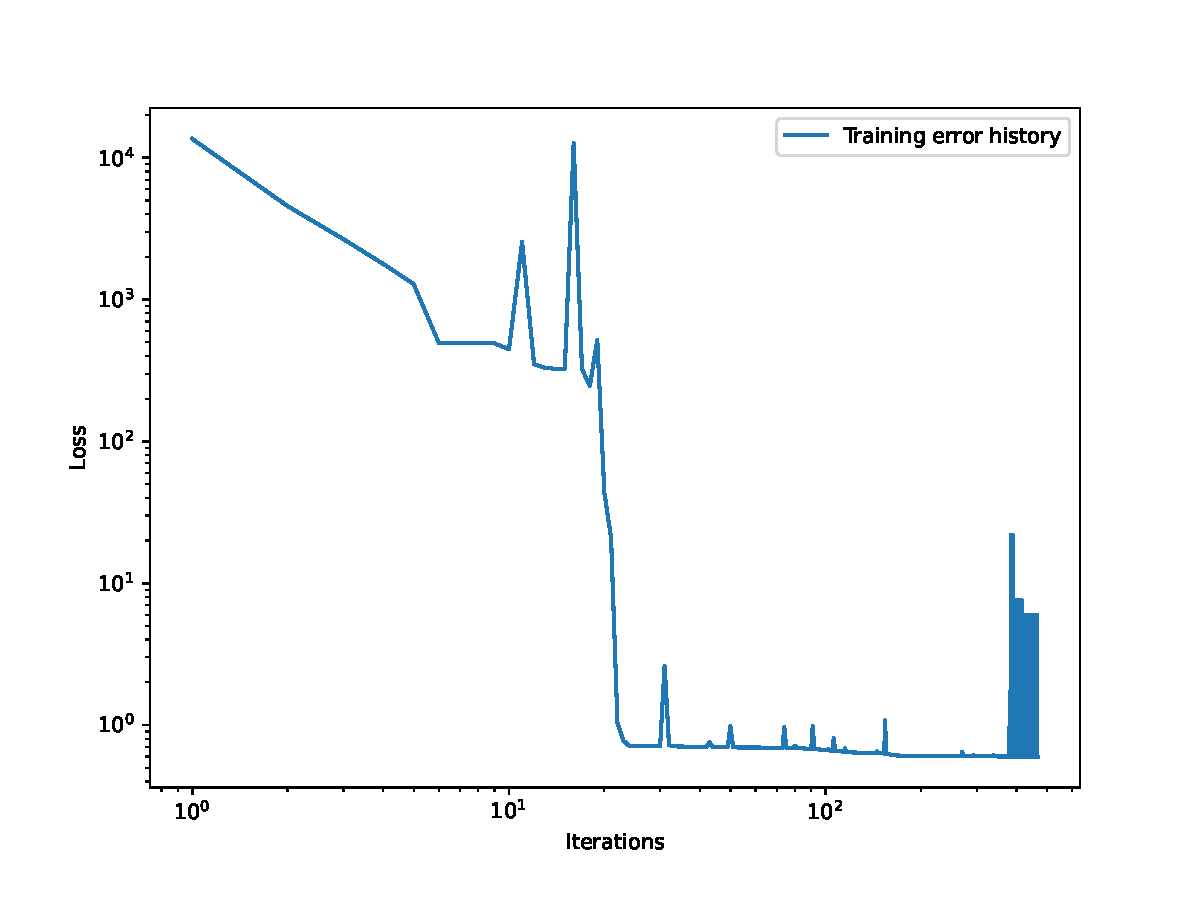
\includegraphics[width=\linewidth]{figures/curve_2/exp_3/history_plot_0.pdf}
        \caption{The cost function \(\mathcal{J}(\theta)\) with each iteration.}\label{fig:curve_2_history}
    \end{subfigure}
    \caption{One approximate solution to the test problem from subsection \ref{subsec:case_2}, found by a neural network and compared with the analytical solution. The corresponding training history is shown in Figure \ref{fig:curve_2_history} }\label{fig:curve_2_example}
\end{figure}

\begin{figure}[b]
    \begin{subfigure}[t]{0.5\textwidth}
        \centering
        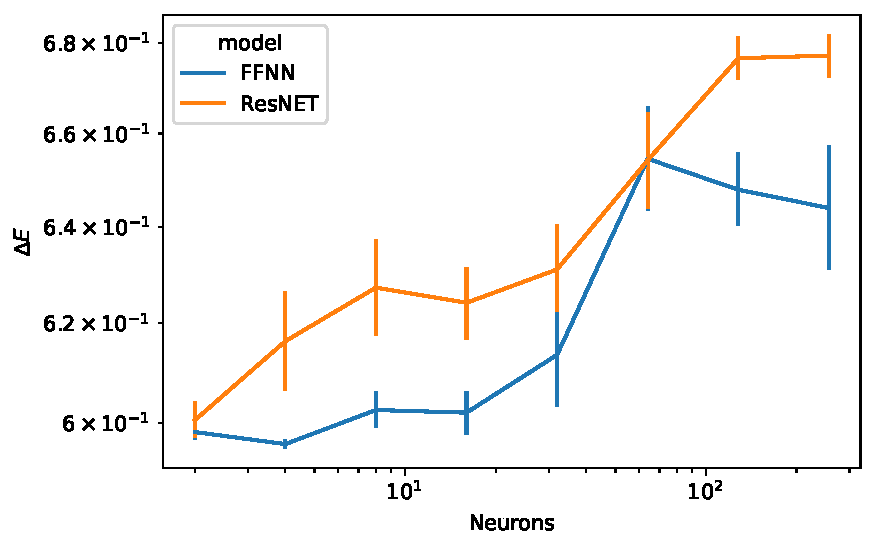
\includegraphics[width=\linewidth]{figures/curve_2/exp_3/neurons_error.pdf}
        \caption{The final cost difference \(\Delta E\) with the number of neurons in each hidden layer.} \label{fig:curve_2_neuron_error}
    \end{subfigure}
    \begin{subfigure}[t]{0.5\textwidth}
        \centering
        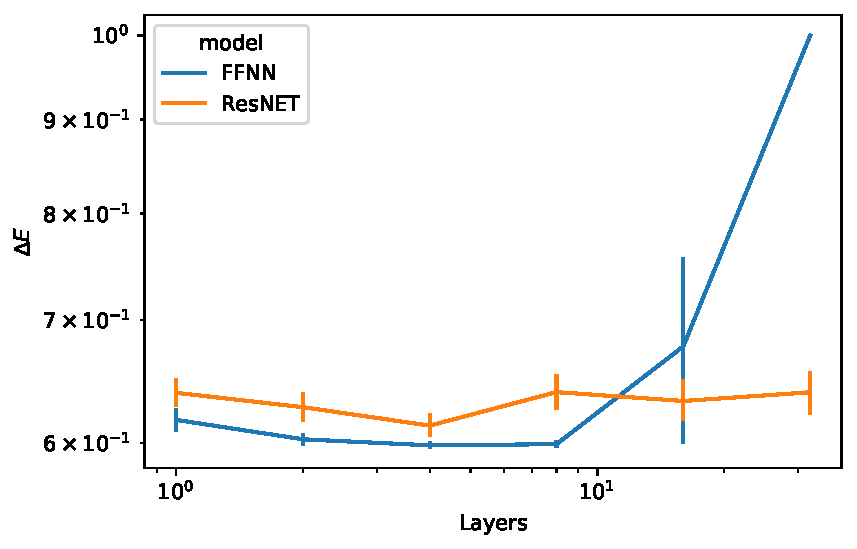
\includegraphics[width=\linewidth]{figures/curve_2/exp_3/layer_error.pdf}
        \caption{Final cost  difference \(\Delta E\) with the number of hidden layers.} \label{fig:curve_2_layer_error}
    \end{subfigure}
    \caption{Result of ensemble training with different number of neurons and hidden layers. The difference between the computed and analytical cost function \(E\) is shown. In Figure \ref{fig:curve_2_neuron_error} the number of layers was fixed at 2. In Figure \ref{fig:curve_2_layer_error} the number of neurons is fixed at 8 per hidden layer. The error bars denote a 80\% confidence interval found by bootstrapping.} \label{fig:curve_2_parmas_eks}
\end{figure}

To test our method, we again performed ensemble training. The result of the ensemble training is shown in Figure \ref{fig:curve_2_parmas_eks}. Also, the resulting reparametrization of the first training is shown in Figure \ref{fig:curve_2_example}. As before, we observe that ResNet outperforms fully connected feedforward networks on large network depths. 
